\subsubsection{A multiplicative-noise example}
\label{subsec:poc-multiplicative}

We next consider the superlinear MV-SDE
\begin{equation}
\label{eq:poc-multiplicative-model}
    \mathrm dX_t
    =
    \left(-2X_t-14X_t^{[3]}+\frac12\mathbb EX_t\right)\mathrm dt
    +S(X_t)\,\mathrm dW_t,
    \qquad X_0\sim\mathcal N(0,I_d),
\end{equation}
where
\[
    S(x):=\operatorname{diag}
    \left(\sqrt{1+x_1^2},\ldots,\sqrt{1+x_d^2}\right),
    \qquad
    x^{[3]}=(x_1^3,\ldots,x_d^3)^{\mathsf T}.
\]
The coefficients satisfy Assumptions~1--4 with
\[
\begin{gathered}
    q_0=80,\qquad \kappa=3,\qquad L=2646,\qquad L_\sigma=1,\\
    K_1=a_1=\frac72,\qquad K_2=a_2=\frac12,\qquad C_0=135d.
\end{gathered}
\]
Indeed, the cubic monotonicity and the estimate
\[
    \left|\sqrt{1+u^2}-\sqrt{1+v^2}\right|^2
    \le\frac13(u^2+uv+v^2)|u-v|^2
\]
allow the diffusion contribution to be absorbed by the cubic drift.
The Gaussian initial distribution has all finite moments.

Simultaneous sign reversal of the initial state and Brownian motion
preserves the equation and the input law, so \(\mathbb EX_t=0\). Thus the non-interacting copies solve
\eqref{eq:poc-multiplicative-model} without the mean-field term.
For the synchronous coupling, let
\[
    u_N(t):=\frac1N\sum_{i=1}^N
    \mathbb E|X_t^{i,N}-X_t^i|^2.
\]
It\^o's formula gives \(\sup_{t\ge0}\mathbb E|X_t^i|^2\le d\).
Using independence of the non-interacting copies and absorbing the
squared diffusion difference into the negative cubic contribution yields
\[
    u_N'(t)\le-\frac52u_N(t)+\frac{d}{2N},\qquad u_N(0)=0.
\]
Consequently, by exchangeability,
\begin{equation}
\label{eq:poc-multiplicative-bound}
    \sup_{t\ge0}\sup_{1\le i\le N}
    \mathbb E|X_t^{i,N}-X_t^i|^2
    \le\frac{d}{5N}.
\end{equation}

We use the same experimental parameters as in the additive-noise example:
\[
\begin{gathered}
    T=100,\qquad h=1/64,\qquad R=64,\\
    d\in\{2,3,4,5,8\},\qquad
    N\in\{40,80,160,320,640,1280,2560\},
\end{gathered}
\]
where \(R\) denotes independent realizations of the entire coupled system.
Both systems are discretized by SSBE. The interacting update is
\[
\left\{
\begin{aligned}
    (1+2h)Z_{n+1}^{i,N}
    +14h(Z_{n+1}^{i,N})^{[3]}
    -\frac h{2N}\sum_{j=1}^NZ_{n+1}^{j,N}
    &=Y_n^{i,N},\\
    Y_{n+1}^{i,N}
    &=Z_{n+1}^{i,N}+S(Z_{n+1}^{i,N})\Delta W_n^i.
\end{aligned}
\right.
\]
The reference scheme omits the empirical mean term and evaluates
\(S\) at its own intermediate value. Each corresponding pair shares
its initial value and Brownian increments
\(\Delta W_n^i\sim\mathcal N(0,hI_d)\). The implicit stages are solved
to a normalized residual tolerance of \(10^{-12}\).
Because the coordinate equations decouple, the lower-dimensional
experiments use coordinate prefixes of the eight-dimensional runs.

At \(n_T=T/h\), the terminal mean-square discrepancy is estimated by
\begin{equation}
\label{eq:poc-multiplicative-error}
    \widehat E_{N,d}(T)
    :=
    \frac1{RN}\sum_{r=1}^R\sum_{i=1}^N
    \left|Y_{n_T}^{i,N,(r)}-\widetilde Y_{n_T}^{i,(r)}\right|^2.
\end{equation}
No square root is taken, and both paths are time-discretized.
Regression using all seven particle numbers gives terminal slopes
\[
    -0.852,\quad -0.890,\quad -0.926,\quad -0.943,\quad -0.957
\]
for \(d=2,3,4,5,8\), respectively.
To reduce the variability associated with a single observation time,
we additionally report the preselected long-time window statistic
\[
    \overline E_{N,d}
    :=\frac1{81}\sum_{j=0}^{80}
    \widehat E_{N,d}(80+j/4).
\]
Its fitted slopes are
\[
    -0.999,\quad -0.996,\quad -0.996,\quad -0.997,\quad -0.995,
\]
respectively. Figure~\ref{fig:poc-multiplicative} displays the terminal
and window-averaged results separately. Markers are observed errors,
solid lines are log--log least-squares fits, and green dashed lines
are proportional to \(N^{-1}\).

At \(N=2560\), a paired stepsize check with 32 independent systems
compares \(h=1/64\) and \(h/2=1/128\). The window-averaged
mean-square discrepancies change by at most \(2.01\%\).
These results support the model-specific long-time \(N^{-1}\)
mean-square estimate. The faster decay relative to the general
PoC upper bound is explained here by the mean-interaction structure;
it is not a verification of sharp dimension-dependent rates.
Finite-horizon observations and reference-grid comparisons do not
by themselves establish an infinite-time bound or eliminate
time-discretization bias.

\begin{figure}[tbp]
    \centering
    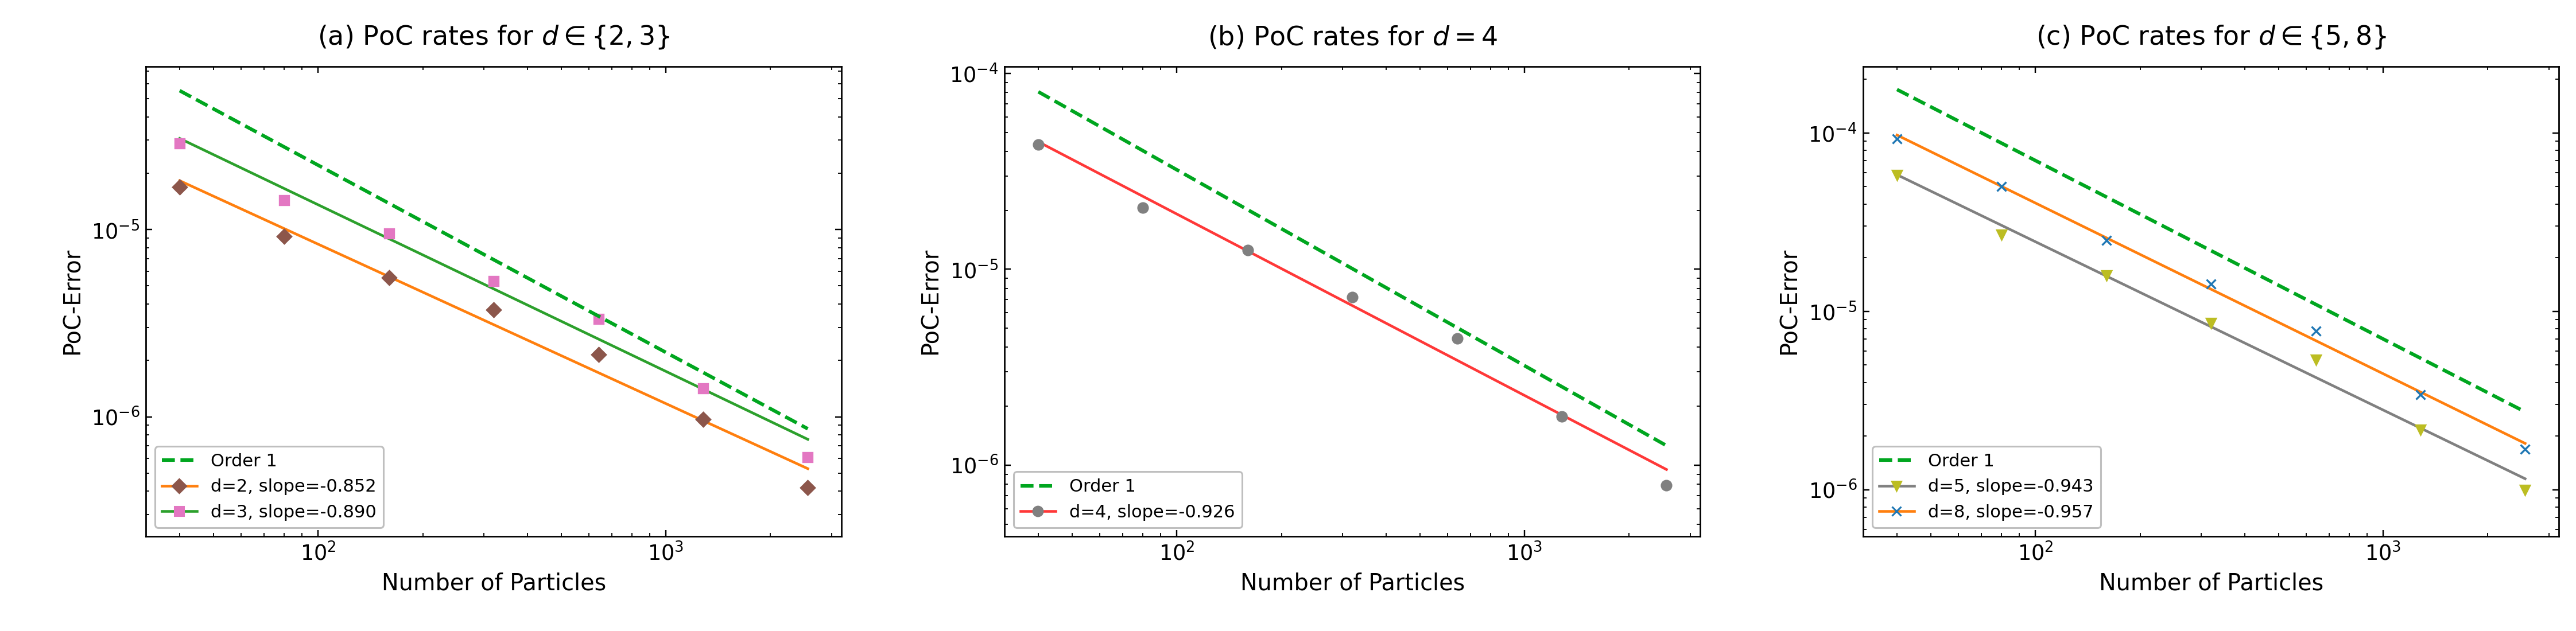
\includegraphics[width=\textwidth]{multiplicative_PoC_T100.png}\\[2mm]
    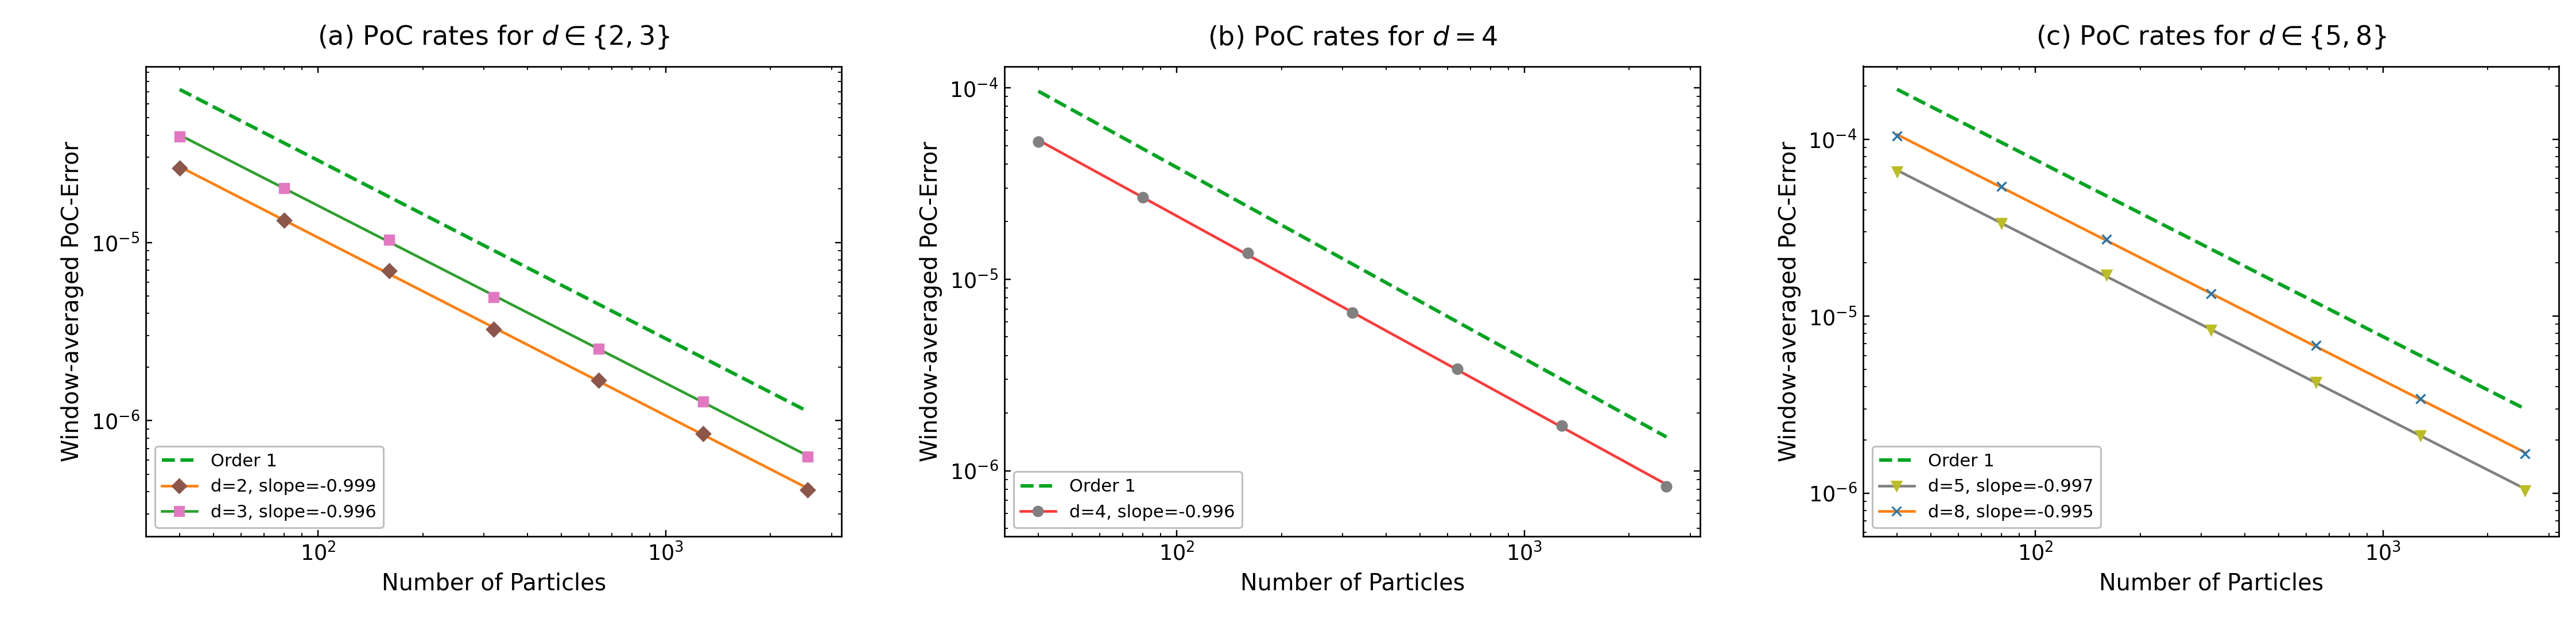
\includegraphics[width=\textwidth]{multiplicative_PoC_window80_100.png}
    \caption{Propagation of chaos for the multiplicative-noise model
    \eqref{eq:poc-multiplicative-model}, with \(h=1/64\) and \(R=64\).
    Top: terminal mean-square discrepancy at \(T=100\).
    Bottom: mean-square discrepancy averaged over the saved times in
    \([80,100]\). In each row, the panels correspond to
    \(d\in\{2,3\}\), \(d=4\), and \(d\in\{5,8\}\).
    The dashed lines indicate an \(N^{-1}\) reference rate.}
    \label{fig:poc-multiplicative}
\end{figure}
